\chapter{引言}

\section{暗物质是什么}
\subsection{暗物质存在的证据:天文观测结果}

\subsection{暗物质的粒子属性:标准模型之外的物理}
暗物质的性质与组成
现有模型的拓展:SUSY supersymmetry 有暗物质候选粒子


\section{暗物质粒子的探测方法}
暗物质粒子探测是当前的科学热点, 具有重要的物理意义和前景, 世界各国都在集中人力、物力和财力研究这一问题。根据目前的技术手段, 探测暗物质粒子的方法大致可以总结为三类: 加速器直接产生法,直接探测法和间接探测法。

加速器直接产生法是发现新粒子最常用和最有效的方法。
利用加速器将粒子加速到高能量进行对撞可以模拟宇宙大爆炸初期环境, 各种新的粒子能够在对撞后产生, 其中也可能包含暗物质候选粒子。
通过对次级粒子的探测或逃逸能量(missing energy)的重建, 可以反推出新粒子的存在并在实验室环境下研究粒子的物理特性。
产生暗物质粒子需要极高的能量, 目前只有欧洲核子中心的大型强子对撞机(LHC)能够满足这个条件。
然而, LHC只能产生较轻的暗物质粒子候选粒子, 对于更重的暗物质候选粒子, 需要建造更高能量的加速器和更加强大的粒子探测器。

第二种是直接探测暗物质粒子。该方法是直接探测来自宇宙空间的暗物质粒子与(探测器上的)原子核碰撞所产生的信号。

第三种间接探测暗物质粒子。间接法是观测暗物质粒子在宇宙空间发生衰变或相互作用之后产生的稳定粒子如伽玛射线、正电子、反质子、中微子等。

\section{暗物质粒子的空间探测}
\subsection{空间探测的优势}

\subsection{国际上的研究现状}

\section{DAMPE暗物质粒子探测卫星}
暗物质粒子子探测卫星 (英文: DArk Matter Particle Explorer, 缩写: DAMPE)是中国科学院首批空间科学战略先导专项之一, 预计于2015年11月在酒泉卫星发射基地由长征二号丁运载火箭发射上空。
DAMPE粒子探测器是暗物质粒子探测卫星的主要载荷, 它是一个高精度宽能段的能谱探测器,专门用来测量空间中高能电子、高能伽玛射线和重离子的能谱和分布。
一旦成功发射, DAMPE粒子探测器将弥补我国在空间暗物质探测上的空白, 同时也将成为世界上覆盖能区最广,精度最高的空间粒子探测器之一。

\subsection{科学目标}
暗物质粒子探测卫星的科学目标可以归结为以下三个方面:
\begin{enumerate}
	\item 寻找暗物质粒子存在的证据, 这是项目的首要目标。 通过在空间高分辨、宽能段地观测高能电子和伽玛射线寻找和研究暗物质粒子,间接测定其质量、湮灭截面或者寿命等重要的物理参量,并限定暗物质粒子的空间分布,在暗物质研究这一前沿科学领域取得重大突破。
	\item 宇宙线物理研究。通过测量TeV以上的高能电子能谱来研究宇宙线起源, 通过测量TeV/核子的核素能谱来研究宇宙射线传播和加速机制。
	\item 伽玛射线天文学研究。通过观测高能伽玛射线在伽玛天文方面取得重要成果。
\end{enumerate}

DAMPE使用间接探测法来研究暗物质粒子。
根据已有的观测结果 (见上节), 高分辨观测高能伽玛射线和电子是探测暗物质粒子可能的突破点。
空间中高能电子和伽玛射线的流量与能量成反比, 且比宇宙线本底(主要是质子和氦核)低百倍以上, 因此如何进行本底抑制是能否这种方法成功的关键。

宇宙线的起源、加速传播机制是天文学中一个重要的研究课题。
高能电子在星际中传播时,会与背景光发生逆康普顿散射且受星际磁场的作用发生同步辐射而损失能量,损失能量的速度与电子能量的平方成正比。
能量越高的电子损失能量越快,所以高能电子不能够传播太远,高于1012eV的高能电子其寿命只有105年,传播距离只有1kpc。
地球附近的宇宙高能电子只能来自于附近的高能电子源,因此它被常用于研究宇宙线的起源。。
宇宙线中的高能ce


DAMPE粒子探测器本身是一个高空间分辨和能量分辨的伽玛射线望远镜,其主要观测能段超过了国际上所有空间伽玛射线望远镜,可能会有许多预见不到的科学发现。如质子衰变实验发现了天体中微子,开辟了中微子天文学这一新的科学领域,这样的例子很多。我们期望本项目观测能够发现许多人类未知的“第一次”。

\begin{table}[htb]
	\centering
	\caption{DAMPE与其它同类探测器的性能比较}
	\label{tab:ch1:dampe_comparison}
	\begin{tabu} to \textwidth{lcccc}
		\toprule[1.5pt]
		  & DAMPE & AMS-02 & FERMI-LAT & CALET \\ 
		\midrule[1pt]
		Energy Range (\si{GeV}) & $5\sim10^4$ & $0.1\sim10^3$ & $0.02\sim300$ & $1\sim10^3$ \\ 
		$e/\gamma$ Energy res.@\si{GeV}(\si{\percent}) & 1.5 & 3 & 10 & 2 \\ 
		$e/\gamma$ Angular res.@\si{GeV}(\si{\degree}) & 0.1 & 0.3 & 0.1 & 0.1 \\ 
		$e/p$ Discrimination& $10^5$ & $10^5\sim10^6$ & $10^3$ & $10^5$ \\ 
		Calorimeter thickness($\Psi_0$) & 31 & 17 & 8.6 & 30 \\ 
		Geometric accep.(\si{\meter\squared\steradian}) & 0.4 & 0.09 & 1 & 0.12 \\ 
		\bottomrule[1.5pt] 
	\end{tabu} 
\end{table}

\subsection{性能指标}
DAMPE卫星将运行于\SI{500}{\kilo\meter}的太阳同步轨道,设计寿命大于三年。
卫星观测能段覆盖5GeV-10TeV,能量分辨优于1.5%,超过国际上所有类似探测器。可望在暗物质粒子探测和宇宙线物理这两大科学难题上取得突破!同时更好的研究伽玛射线天文学等相关重要科学问题。
\subsection{DAMPE粒子探测器的组成}
DAMPE粒子探测器由四个子探测器系统组成, 分别是塑闪阵列探测器, 硅迳迹探测器, BGO量能器和中子探测器, 见图\ref{fig:dampe_structure}。
下面分别对各子探测器进行简单的介绍。

BGO量能器(BGO Calorimeter, 简称:BGO)

塑闪阵列探测器(Plastic Scintillator Array Detector, 简称:PSD)
塑闪阵列探测器是DAMPE的关键子探测器之一,它的主要功能有两点:
\begin{enumerate}
	\item 协助BGO量能器区分光子事件和电子事件。
	\item 鉴别入射重离子的种类,作为硅阵列探测器电荷测量的备份。
\end{enumerate}

硅迳迹探测器(Silicon-Tungsten Tracker, 简称:STK)

中子探测器(Neutron Detector, 简称:NUD)

\begin{figure}
\centering
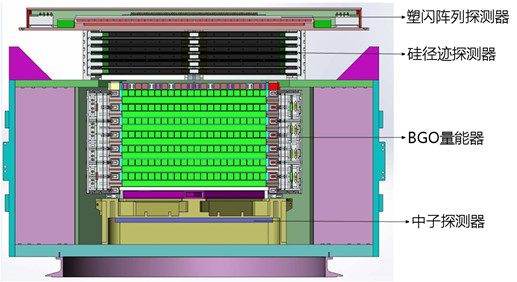
\includegraphics[width=0.8\linewidth]{chap/introduction/fig/dampe_structure_2}
\caption{DAMPE暗物质粒子探测器的整体结构}
\label{fig:dampe_structure}
\end{figure}
